\documentclass[tikz,border=3pt]{standalone}
\begin{document}
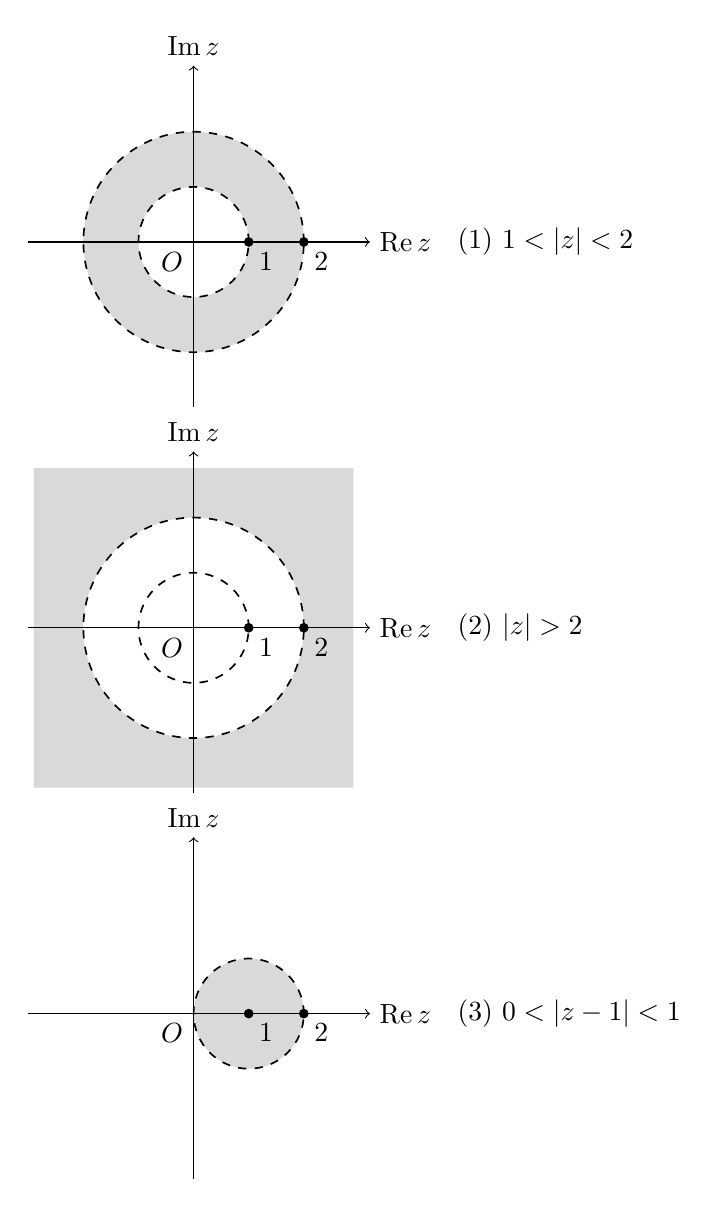
\begin{tikzpicture}[scale=0.7,line width=0.9pt]
  \foreach \k/\dy/\lab in {1/0/{(1)\ $1<|z|<2$},2/-7/{(2)\ $|z|>2$},3/-14/{(3)\ $0<|z-1|<1$}}{
    \begin{scope}[yshift=\dy cm]
      \ifnum\k=1
        \fill[black!15,even odd rule] (0,0) circle (2) (0,0) circle (1);
      \fi
      \ifnum\k=2
        \fill[black!15,even odd rule] (-2.9,-2.9) rectangle (2.9,2.9) (0,0) circle (2);
      \fi
      \ifnum\k=3
        \fill[black!15] (1,0) circle (1);
      \fi
      \draw[line width=0.4pt,->] (-3,0) -- (3.2,0) node[right] {$\mathrm{Re}\,z$};
      \draw[line width=0.4pt,->] (0,-3) -- (0,3.2) node[above] {$\mathrm{Im}\,z$};
      \node[below left] at (0,0) {$O$};
      \ifnum\k<3
        \draw[dashed,line width=0.6pt] (0,0) circle (1);
        \draw[dashed,line width=0.6pt] (0,0) circle (2);
      \else
        \draw[dashed,line width=0.6pt] (1,0) circle (1);
      \fi
      \fill (1,0) circle (2.5pt);
      \fill (2,0) circle (2.5pt);
      \node[below right] at (1,0) {$1$};
      \node[below right] at (2,0) {$2$};
      \node[right] at (4.6,0) {\lab};
    \end{scope}}
\end{tikzpicture}
\end{document}
